\question (西安理工大学)双端口存储在( )情况下会发生读/写冲突
\par\twoch{左端口与右端口的地址码不同}{\textcolor{red}{左端口与右端口的地址码相同}}{左端口与右端口的数据码相同}{左端口与右端口的数据码不同}
\begin{solution}B。
这里只能选择最佳答案,其实B选项也是有漏洞的。对于一个双端口存储器,两个端口是可以对同一地址的单元进行读操作的,这不算冲突。只有对同一地址的单元同时进行写操作时,才算冲突。
\end{solution}
\question 下列关于存储器的说法中,正确的有
Ⅰ.多体交叉存储器是按低地址作为区分存储器的标记的
Ⅱ.存储系统中主要通过并行主存储器和设置Cache来提高速度
Ⅲ.LRU替换算法的平均命中率要高于FIFO替换算法的平均命中率
Ⅳ.页式管理的虚拟存储器,按地址访问的页表称为``快表''
\par\twoch{Ⅰ和Ⅱ}{Ⅰ、Ⅲ和Ⅳ}{Ⅱ}{\textcolor{red}{Ⅱ和Ⅲ}}
\begin{solution}D。
I错误。多体交叉存储器一旦给出存储器地址,存储器模块会按每个周期回送一个字。如果对不同的存储器模块给定不同的地址,则可以同时对多个字进行存取,或以流水线方式对它们进行存取,这样的存储器叫做多体交叉存储器。它又分为低位交叉存取和高位交叉存取两种形式。
·低位交叉存取:将邻接的存储器单元沿横向放在m个模块中。这意味着存储器地址的低位用来指明存储器模块,高位则是每个模块内的字地址。
·高位交叉存取:用高位作为模块地址,用低位作为每个模块内的字地址。
所以多体交叉存储器不都是按低地址作为区别存储器的标记的。故Ⅰ错误。
Ⅱ正确。这正是存储系统提高速度常用的两种方法。
Ⅲ正确。LRU替换算法的平均命中率一般是要高于FIFO替换算法的平均命中率。因为LRU算法反映了程序的局部性特点。
Ⅳ错误。快表的定义是这样的:由于程序局部性的特点,对页表内部各行的使用不是随机的,而是簇聚在一起的。就是说,在一段时间内只使用了表中的很少的几行。这样可以使用一个比全部的页表的内容少很多的目录表,也就是快表,来提高查找的速度。快表也称为TLB,它是内存中页表的一小部分,用相联存储器实现。它是按内容访问的,而按地址访问的页表是慢表。
综上所述,只有Ⅱ和Ⅲ是正确的。
\end{solution}
\question 设存储器容量为32字,字长为64位。模块数m=4,采用低位交叉方式。存储周期T=200ns,数据总线宽度为64位,总线传输周期r=50ns。该交叉存储器的带宽是
\par\fourch{bit/s}{bit/s}{\textcolor{red}{bit/s}}{bit/s}
\begin{solution}C。
在低位交叉存储器中,连续的地址分布在相邻的块中,而同一模块内的地址都是不连续的。这种存储器采用分时启动的方法,可以在不改变每个模块存取周期的前提下,提高整个主存的速度。
低位交叉存储器连续读出4个字所需的时间为t=T+(m-1)*r=200ns+3*50ns=350ns=
3.5*10\^{}-7s。故带宽为W=64*4bit/(3.5*10\^{}-7s)=73×10\^{}7bit/s。
\end{solution}
\question 采用八体并行低位交叉存储器,设每个体的存储容量为32K×16位,存取周期为400ns,下述说法中正确的是
\par\fourch
{\textcolor{red}{在400ns内,存储器可向CPU提供$2^7$位二进制信息}}
{在100ns内,每个体可向CPU提供$2^7$位二进制信息}
{在400ns内,存储器可向CPU提供$2^8$位二进制信息}
{在100ns内,每个体可向CPU提供$2^8$位二进制信息}
\begin{solution}A。
计算过程:八体并行低位交叉存储器,存取周期和总线周期需要满足存取周期=8×总线周期,因此得到总线周期为50ns。对于单个个体而言,每个存取周期内仍然只能取出16位,但是由于CPU交叉访问8个存储体,所以可以在一个存取周期内使得8个存储体各传输16位,共16×8=128位,也就是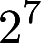
\includegraphics[width=0.15625in,height=0.15625in]{texmath/a136d35Cdpi7B3507D25E7}位二进制信息。
\end{solution}
